



\section{Đánh giá hiệu năng hệ thống nhúng}

Triển khai học máy tại biên (\textit{TinyML}) vào sản xuất công nghiệp không chỉ đánh giá dựa trên độ chính xác thuật toán mà còn phụ thuộc vào hiệu năng thực thi trên phần cứng giới hạn. Độ trễ, mức tiêu thụ bộ nhớ và độ ổn định của hệ điều hành thời gian thực (RTOS) là tiêu chí đánh giá tính khả thi của hệ thống \cite{ref_mlperf_tiny}.

\subsection{Phân tích độ trễ suy luận}

Độ trễ suy luận là thời gian từ khi vi điều khiển hoàn tất trích xuất đặc trưng đầu vào (vectơ 19 chiều) cho đến khi đưa ra sai số tái tạo MAE và nhãn phân loại. Duy trì độ trễ suy luận thấp giúp hệ thống phản ứng tức thời với các sự cố cơ khí đột ngột trước khi gây thiệt hại vật lý.

Nhờ lượng tử hóa nhận thức huấn luyện chuyển đổi trọng số sang INT8, hệ thống tối ưu hóa khối lượng tính toán. Bên cạnh đó, Seeed Studio XIAO ESP32-S3 sở hữu kiến trúc lõi kép Xtensa® LX7 tích hợp tập lệnh vector SIMD chuyên dụng cho trí tuệ nhân tạo, thực thi song song các phép toán nhân-tích lũy (MAC) trên mảng dữ liệu \cite{ref_1_15, ref_1_7}.

Để đo đạc chính xác, hệ thống thực hiện đánh giá hiệu năng tự động với N=1\,000 lần suy luận trên từng mô hình, sử dụng hàm \texttt{esp\_timer\_get\_time()} đo trực tiếp thời gian thực thi của hàm \texttt{Invoke()} trong TensorFlow Lite Micro. Kết quả cho thấy thời gian suy luận trung bình tổng hợp đạt \textbf{6,44 ms} (Bảng~\ref{tab:latency_stats}).

\begin{table}[H]
\centering
\caption[Thống kê độ trễ suy luận]{Thống kê độ trễ suy luận trên vi điều khiển Seeed Studio XIAO ESP32-S3 (N=1\,000 mẫu mỗi mô hình, tổng cộng 3\,000 phép đo)}
\label{tab:latency_stats}
\begin{tabular}{|l|c|c|c|c|c|c|}
\hline
\textbf{Mô hình} & \textbf{Mean ($\mu s$)} & \textbf{Std} & \textbf{Min} & \textbf{Max} & \textbf{P95} & \textbf{P99} \\ \hline
GENTLE & 6.411 & 71,9 & 6.274 & 6.536 & 6.516 & 6.526 \\ \hline
STRONG & 6.512 & 21,0 & 6.449 & 6.552 & 6.543 & 6.551 \\ \hline
SPIN   & 6.393 & 20,3 & 6.344 & 6.438 & 6.427 & 6.429 \\ \hline
\rowcolor[HTML]{EFEFEF}
\textbf{Tổng hợp} & \textbf{6.439} & \textbf{68,8} & \textbf{6.274} & \textbf{6.552} & \textbf{6.535} & \textbf{6.545} \\ \hline
\end{tabular}
\end{table}

\begin{figure}[H]
    \centering
    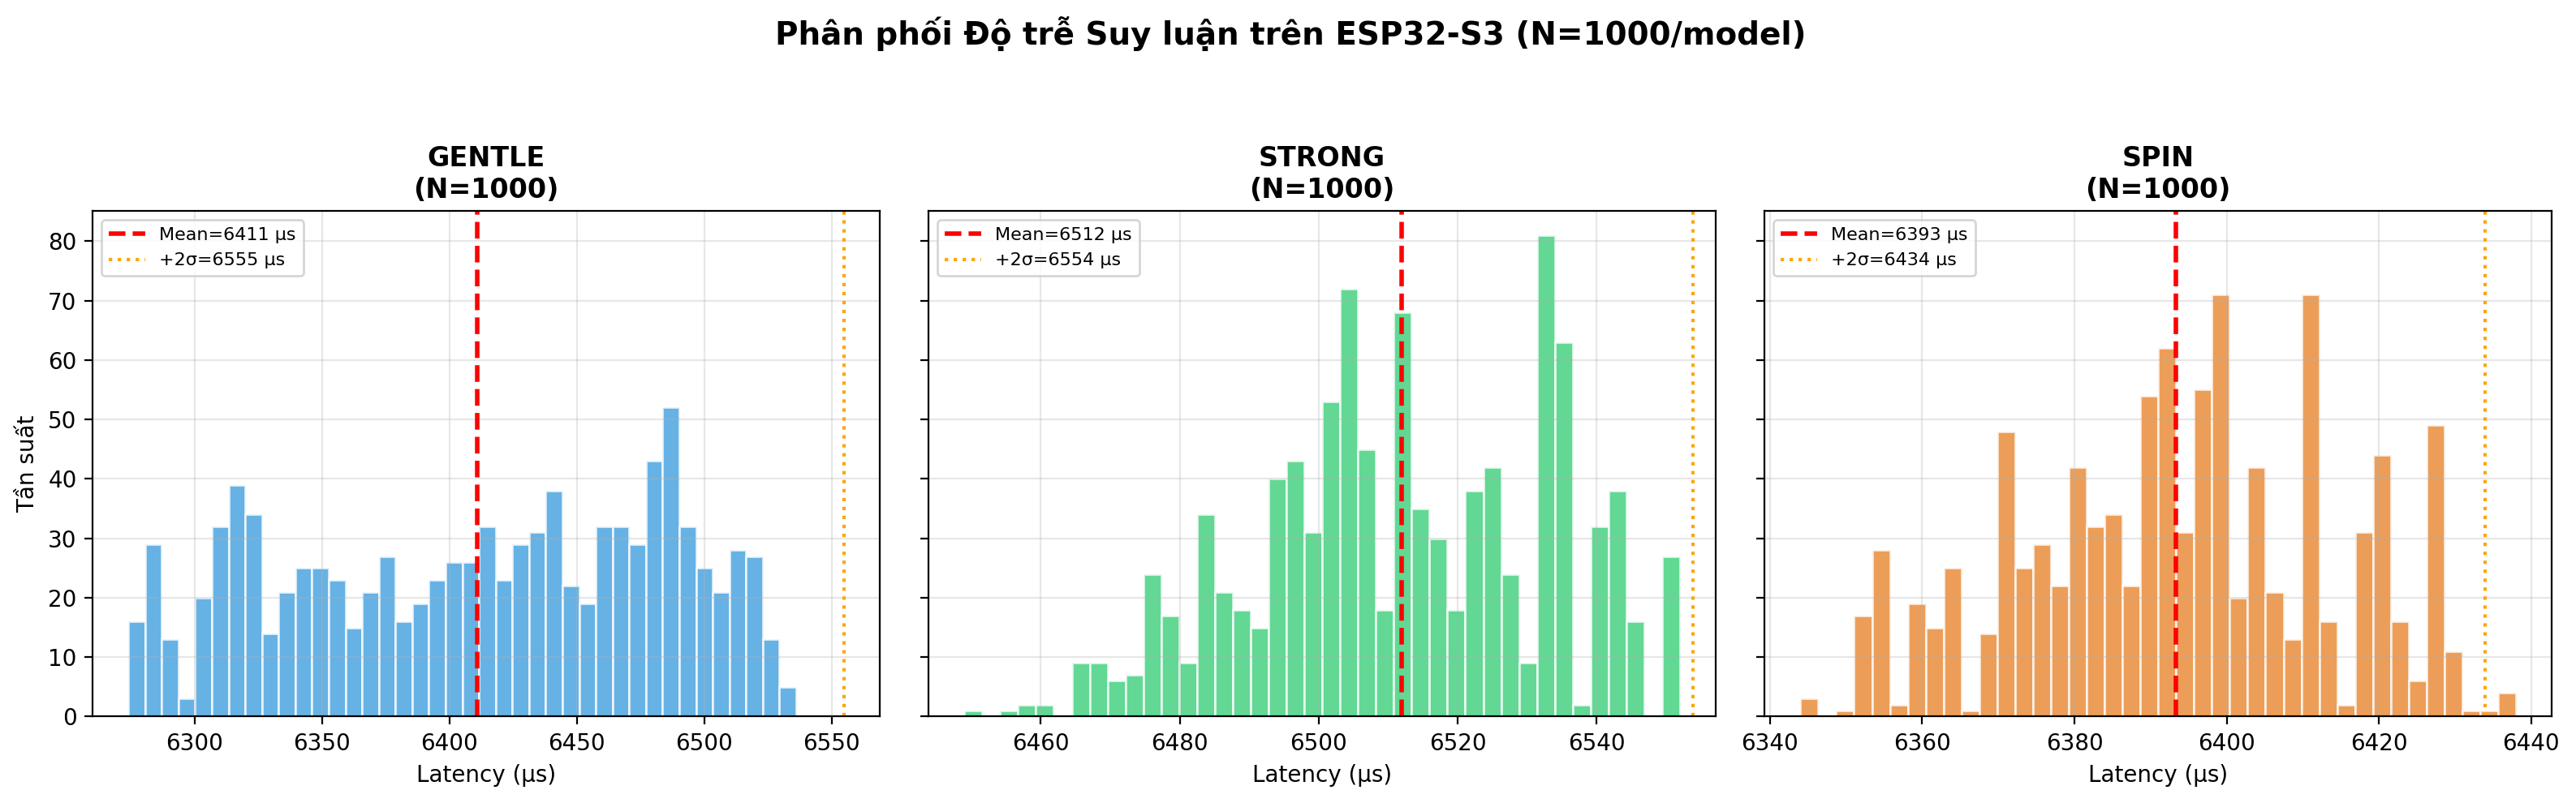
\includegraphics[width=0.95\linewidth]{chap4/image/latency_histogram.png}
    \caption[Phân phối độ trễ suy luận]{Biểu đồ phân phối thực nghiệm của độ trễ suy luận trên vi điều khiển Seeed Studio XIAO ESP32-S3 cho 3 mô hình ba trạng thái. Mỗi mô hình được đo 1\,000 lần suy luận liên tiếp. Độ trễ tập trung ổn định quanh 6,4 ms với độ lệch chuẩn thấp ($< 72 \mu s$).}
    \label{fig:latency_histogram}
\end{figure}

\begin{itemize}
    \item Đánh giá đáp ứng thời gian thực: Với tần số lấy mẫu đặc trưng 1 Hz (chu kỳ 1\,000 ms), thời gian suy luận 6,4 ms chỉ chiếm $0{,}64\%$ quỹ thời gian CPU, dư dả cho các tác vụ khác.
    \item Dư địa tài nguyên: Tác vụ Trí tuệ nhân tạo (AI) hoàn thành trong vài mili-giây, cho phép lõi CPU số 1 nhường tài nguyên cho các tác vụ giao tiếp mạng (MQTT, TLS/SSL) mà không gây nghẽn cổ chai.
    \item Biến động thời gian suy luận: Mô hình GENTLE ghi nhận độ lệch chuẩn cao hơn so với hai mô hình còn lại. Điều này xuất phát từ việc vùng đệm tensor được cấp phát trên PSRAM ngoại vi; các hiện tượng trượt bộ nhớ đệm ngẫu nhiên của vi điều khiển Seeed Studio XIAO ESP32-S3 khi truy xuất dữ liệu qua bus SPI làm tăng nhẹ thời gian của một số chu kỳ. Tuy nhiên, mức chênh lệch này vẫn nằm trong ngưỡng chấp nhận được của hệ thống.
\end{itemize}

\subsection{Đánh giá mức sử dụng tài nguyên bộ nhớ và độ ổn định hệ thống}

Rào cản chính khi đưa các mô hình Học sâu vào vùng biên là dung lượng bộ nhớ tĩnh (Flash) và động (SRAM) eo hẹp \cite{ref_1_7, ref_1_4}.

\textbf{Chiếm dụng bộ nhớ Flash và số lượng tham số:} \\
Hệ thống tối ưu hóa kiến trúc đối xứng với Lớp thắt cổ chai 32 chiều và lượng tử hóa INT8 triệt để. Toàn bộ 3 mô hình (GENTLE, STRONG, SPIN) sau lượng tử hóa INT8 có tổng dung lượng chỉ \textbf{95,3 KB}. Khi tích hợp vào firmware hoàn chỉnh (mã điều khiển, FreeRTOS, TensorFlow Lite for Microcontrollers, thư viện MQTT/TLS, WiFi stack và các driver I2S/I2C), tổng dung lượng Flash được ghi nhận qua kết quả biên dịch thực tế là \textbf{1.254.517 bytes} (xấp xỉ \textbf{1,20 MB}), chiếm \textbf{37\%} không gian chương trình (Hình~\ref{fig:flash_usage}).

\begin{figure}[H]
    \centering
    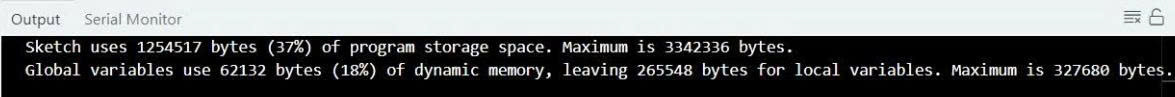
\includegraphics[width=0.85\linewidth]{chap4/image/flash_usage_proof.png}
    \caption[Kết quả biên dịch firmware]{Kết quả biên dịch firmware v11 trên Arduino IDE 2.3.5, xác nhận mức chiếm dụng bộ nhớ Flash (37\%) và SRAM (18\%) thực tế trên vi điều khiển Seeed Studio XIAO ESP32-S3.}
    \label{fig:flash_usage}
\end{figure}

\textbf{Quản lý bộ nhớ động (SRAM/PSRAM):} \\
TensorFlow Lite Micro đòi hỏi vùng nhớ đệm để lưu trữ các tensor trung gian. Nhờ kiến trúc gọn nhẹ, tổng không gian nhớ mà các mô hình yêu cầu rất thấp. Bộ nhớ động (Global Variables) chiếm \textbf{62.132 bytes (18\%)} trên tổng 327.680 bytes SRAM, để dư 265.548 bytes cho các tác vụ thời gian thực. Hệ thống quy hoạch bộ nhớ trên kiến trúc lõi kép Seeed Studio XIAO ESP32-S3:
\begin{enumerate}
    \item Tận dụng SRAM nội bộ (512 KB) cho các bộ đệm DMA tốc độ cao của cảm biến âm thanh và rung động để tránh mất mẫu.
    \item Vùng nhớ (3 × 40 KB) được cấp phát trên PSRAM 8 MB thông qua hàm \texttt{heap\_caps\_aligned\_alloc()}, đảm bảo dư dả tài nguyên cho các tác vụ giao tiếp mạng mà không gây xung đột hay Tràn ngăn xếp.
    \item Hệ thống có thể duy trì hoạt động liên tục trong nhiều chu kỳ giặt mà không xảy ra Rò rỉ bộ nhớ hay Watchdog Reset.
\end{enumerate}

Độ ổn định hệ thống trong thử nghiệm thực địa: \\
Hệ thống được đánh giá qua các bài kiểm tra thực địa kéo dài nhiều chu kỳ hoạt động đầy đủ của máy giặt. Nhờ kiến trúc FreeRTOS đa nhiệm:
\begin{itemize}
    \item Tác vụ thu thập cảm biến trên lõi số 0 và tác vụ suy luận Trí tuệ nhân tạo trên lõi số 1 hoạt động độc lập thông qua Nhóm sự kiện và Hàng đợi.
    \item Tình trạng tác vụ không được cấp đủ thời gian CPU và xung đột tài nguyên được ngăn chặn nhờ gán mức độ ưu tiên (ví dụ: ngắt I2C đo rung động được cấp mức ưu tiên 15 - cao nhất để đảm bảo thời gian thực).
\end{itemize}
Trong các thử nghiệm dài hạn, hệ thống không ghi nhận Rò rỉ bộ nhớ hay Watchdog Reset. Dữ liệu đo xa được duy trì ổn định ở tần suất 1,0 Hz, đảm bảo luồng dữ liệu mượt mà cho cơ chế lọc nhiễu cửa sổ thời gian và kích hoạt cảnh báo tức thời trên ứng dụng di động.
